\makeatletter
\def\input@path{{../styles/}{../../styles/}{../../../styles/}{../}{../../}{../../../}}
\makeatother
\documentclass{ee102_notes}
% macros.tex - Course meta information
\renewcommand{\course}{EE 102}
\renewcommand{\coursetitle}{Signal Processing and Linear Systems}
\renewcommand{\instructor}{Ayush Pandey}
\renewcommand{\semester}{Fall}
\renewcommand{\year}{2025}
\renewcommand{\shorttitle}{Week 1: Introduction to Signals}
% Use \renewcommand to avoid 'already defined' errors

% The following packages can be found on http:\\www.ctan.org
% \usepackage{graphics} % for pdf, bitmapped graphics files
%\usepackage{epsfig} % for postscript graphics files
%\usepackage{mathptmx} % assumes new font selection scheme installed
%\usepackage{times} % assumes new font selection scheme installed
\usepackage{amsmath} % assumes amsmath package installed
\usepackage{amssymb,mathtools}  % assumes amsmath package installed
\usepackage{xcolor}
\usepackage{pgfplots,subcaption}
\usepackage[hidelinks]{hyperref}
\usepackage{verbatim}
\usepackage{graphicx}
\usepackage{listings}
\usepackage{fancyhdr}
% \usepackage{geometry}
\usepackage{siunitx}
\usepackage[most]{tcolorbox}
\usepackage{enumitem}
\usepackage{environ}
% -------- listings (Python) ----------
\lstdefinestyle{py}{
  language=Python,
  basicstyle=\ttfamily\small,
  keywordstyle=\color{blue!60!black}\bfseries,
  commentstyle=\color{green!40!black},
  stringstyle=\color{orange!60!black},
  showstringspaces=false,
  columns=fullflexible,
  frame=single,
  framerule=0.3pt,
  numbers=left,
  numberstyle=\tiny,
  xleftmargin=1em,
  tabsize=2,
  breaklines=true,
}

\usepackage[american]{circuitikz}
\usepackage{tikz}
\usetikzlibrary{arrows.meta,positioning,calc,angles,quotes}
\tikzset{
  >={Latex[length=2.2mm]},
  block/.style={draw, thick, rectangle, minimum height=10mm, minimum width=24mm, align=center},
  gain/.style={block, minimum width=14mm},
  sum/.style={draw, thick, circle, inner sep=0pt, minimum size=6mm},
  conn/.style={-Latex, thick},
}
\usepackage{caption}    
\usepackage{lscape}
\usepackage{soul}
\usepackage{physics}
\usepackage{hyperref}
\hypersetup{
    colorlinks=true,
    linkcolor=blue,
    filecolor=magenta,      
    urlcolor=blue,
    pdftitle={week1_notes},
    pdfpagemode=FullScreen,
}
%\usepackage{float} 

%\usepackage[demo]{graphicx}
\pgfplotsset{compat=1.18}
% \usepgfplotslibrary{fillbetween}

\newsavebox{\measurebox}

\let\proof\relax\let\endproof\relax


\def\abs#1{\left\lvert#1\right\rvert}
\let\proof\relax
\let\endproof\relax
\usepackage{amsthm}
\usepackage{accents}
\usepackage{relsize}
\newcommand{\ubar}[1]{\underaccent{\bar}{#1}}
\newtheorem{theorem}{Theorem}
\newtheorem{corollary}{Corollary}[theorem]
\newtheorem{lemma}{Lemma}
\newtheorem{proposition}{Proposition}
\newtheorem{statement}{Statement}

\theoremstyle{definition}
\newtheorem{definition}{Definition}
 
\theoremstyle{remark}
\newtheorem*{remark}{Remark}
\theoremstyle{remark}
\newtheorem*{claim}{Claim}
\setlength{\parindent}{0cm}
\newenvironment{nalign}{
    \begin{equation}
    \begin{aligned}
}{
    \end{aligned}
    \end{equation}
    \ignorespacesafterend
}

\renewcommand{\releasedate}{September 10, 2025}
\begin{document}

\section*{EE 102 Week 2, Lecture 2 (Fall 2025)}
\subsection*{Instructor: \instructor}
\subsection*{Date: \releasedate}
\section{Goals}
\begin{itemize}
    \item The timeless trio of signals: the complex exponential, the unit step, and impulse.
    \item The unit step function as a switch and an accumulator.
    \item The unit impulse function as an exciter and a sampler.
    \item The complex exponential signal as a sinusoid and a phasor.
    \item Applications of the timeless trio in real-world signal processing.
\end{itemize}
\section{The unit step function}
When we defined signals informally, we discussed how any mathematical function from your calculus class could be a signal as long as it represents something physical. Then it will not come as a surprise that for physical system applications, we would usually be interested only in positive values of time and we would want our signal to take the value of zero for all $t < 0$. Since we are extending the general concept of mathematical functions (which are defined for all $t$), it is important to have a mathematical way to write signals that are zero for $t < 0$. The unit step function does exactly that! Formally, we define the unit step function as
\begin{definition}
The unit step is a function defined as
\[
u(t) = \begin{cases}
1, & t \geq 0 \\
0, & t < 0
\end{cases}.
\]
\end{definition}

\subsection{The unit step as a switch}
As you can see in Figure~\ref{fig:unit_step}, it is a discontinuous function that ``steps'' from 0 to 1 at $t = 0$. You may find the unit step function with different names: like the Heaviside function, or the ultrasensitive switch function. 
% add a tikz figure of unit step function
\begin{figure}[h!]
    \centering
    \begin{tikzpicture}
        \begin{axis}[
            axis lines=middle,
            xlabel={$t$},
            ylabel={$u(t)$},
            xtick={-2,-1,0,1,2},
            ytick={0,1},
            ymin=-0.5, ymax=1.5,
            xmin=-2.5, xmax=2.5,
            grid=both,
            width=10cm,
            height=6cm,
            domain=-2.5:2.5,
            samples=1000,
        ]
        \addplot[thick,blue] {x < 0 ? 0 : 1};
        \draw[dashed] (axis cs:0,0) -- (axis cs:0,1);
        \end{axis}
    \end{tikzpicture}
    \caption{The unit step function $u(t)$.}
    \label{fig:unit_step}
\end{figure}

So, any function that is zero for $t < 0$ can be written as the product of the unit step function and another function that defines the behavior of the signal for $t \geq 0$. For example, if we have a signal that is zero for $t < 0$ and equals $f(t)$ for $t \geq 0$, we can write it as $x(t) = f(t)u(t)$.
\subsection{Example: A sinusoidal audio wave that starts at zero time}
If $f(t) = A sin(\omega t + \phi)$, then we can write the signal as 
\[
x(t) = A \sin(\omega t + \phi) u(t).
\]
This signal is zero for $t < 0$ and equals a sinusoidal wave for $t \geq 0$. The unit step function effectively ``switches on'' the sinusoidal wave at $t = 0$. 
But did we \emph{really} need the step function here? You can argue that we could have defined all signals using two cases, 
\[
x(t) = \begin{cases}
f(t), & t \geq 0 \\
0, & t < 0
\end{cases}
\]
but this type of definition will quickly get cumbersome. So, yet again, we are introducing a mathematical object to make our lives easier, at least in the long run (at the moment, it may seem that we are making our life harder by learning another new function).
For the specific sinusoidal example, the alternative way to define it is using a piecewise function that would need two different cases:
\[
x(t) = \begin{cases}
0, & t < 0 \\
A \sin(\omega t + \phi), & t \geq 0
\end{cases}.
\]
We would prefer $x(t) = A \sin(\omega t + \phi) u(t)$ over the piecewise definition so that we can work with just a single expression. 
\subsection{Unit step as a general switch}
Beyond the switching behavior of unit step, we can also use it to define arbitrary ``pulse'' signals and also other piecewise continuous signals. For example, we can define a rectangular pulse of width $\tau$ as
\[
p_\tau(t) = u(t) - u(t - \tau).
\]
This pulse is 1 for $0 \leq t < \tau$ and zero otherwise (can you prove this without relying on sketching?). It is also possible to write the equation of the pulse signal by using a time reversal: 
\[
p_\tau(t) = u(t) + u(\tau - t) - 1
\]
The sketch in both cases is the same: a pulse that starts at $t = 0$ and ends at $t = \tau$. More generally, we can write a pulse that starts at $t_1$ and ends at $t_2$ as
\[
p_{t_1,t_2}(t) = u(t - t_1) - u(t - t_2).
\]
See Figure~\ref{fig:rect_pulse} for a sketch of the rectangular pulse that starts at $t_1$ and ends at $t_2$.
\begin{figure}[h!]
  \centering
  % numeric locations (for drawing); labels will show 0, t_1, t_2 only
  \def\tOne{1}
  \def\tTwo{3}
  \begin{tikzpicture}
    \begin{axis}[
      axis lines=middle,
      xlabel={$t$},
      ylabel={$p_{t_1,t_2}(t)$},
      xtick={0},                         % show only 0 as a regular tick
      extra x ticks={\tOne,\tTwo},       % add ticks at t1 and t2
      extra x tick labels={$t_1$,$t_2$}, % label them symbolically
      ytick={0,1},
      ymin=-0.5, ymax=1.5,
      xmin=-2.5, xmax=4.5,
      grid=both,
      width=10cm,
      height=6cm,
      domain=-2.5:4.5,
      samples=800,
    ]
      % rectangular pulse: 1 on [t1, t2), else 0
      \addplot[thick,blue] {(x >= \tOne) * (x < \tTwo)};
      % dashed guides at t1 and t2
      \draw[dashed] (axis cs:\tOne,0) -- (axis cs:\tOne,1);
      \draw[dashed] (axis cs:\tTwo,0) -- (axis cs:\tTwo,1);
    \end{axis}
  \end{tikzpicture}
  \caption{A rectangular pulse $p_{t_1,t_2}(t)$ that is 1 for $t\in[t_1,t_2)$ and 0 otherwise.}
  \label{fig:rect_pulse}
\end{figure}


The pulse function provides us with more control over when the signal ``turns on'' and ``turns off'' --- in Figure~\ref{fig:rect_pulse}, it turns on at $t = t_1$ and turns off at $t = t_2$. We would expect such knobs of any modern switching system!

We can also define a triangular pulse of width $2\tau$ that is zero for all $t < 0$ and $t > 2\tau$, and peaks at $t = \tau$. This triangular pulse would increase linearly from 0 to 1 in the interval $[0, \tau]$ and then decrease linearly from 1 to 0 in the interval $[\tau, 2\tau]$. By writing the equations of the two linear segments and then combining with unit step to decide when would each linear segment be ``active'', we can write the equation of the triangular pulse. Let's build it step-by-step. We write the two parts that ``activate'' the two linear segments using unit step functions:
\[
w_1(t)=\underbrace{u(t)-u(t-\tau)}_{\text{active on }[0,\tau)},\qquad
w_2(t)=\underbrace{u(t-\tau)-u(t-2\tau)}_{\text{active on }[\tau,2\tau)}.
\]
now, we define the two linear segments:
% Step 2: define the linear pieces (rise and fall)
\[
r(t)=\underbrace{\frac{t}{\tau}}_{\text{linear rise}},\qquad
f(t)=\underbrace{2-\frac{t}{\tau}}_{\text{linear fall}}.
\]
Then, the triangular pulse is obtained by gating each linear segment with its corresponding window and then adding the two gated segments:
% Step 3: gate each piece with its window, then add
\[
tr_\tau(t)
=\underbrace{r(t)}_{\text{rise}}\;\underbrace{w_1(t)}_{\text{gate }[0,\tau)}
+\underbrace{f(t)}_{\text{fall}}\;\underbrace{w_2(t)}_{\text{gate }[\tau,2\tau)}.
\]

% Expanded (single-line) version remove underbraces
\[
tr_\tau(t)
=\frac{t}{\tau}\big[u(t)-u(t-\tau)\big]
+\left(2-\frac{t}{\tau}\right)\big[u(t-\tau)-u(t-2\tau)\big].
\]
See Figure~\ref{fig:tri_pulse} for a sketch of the triangular pulse.
\begin{figure}[h!]
  \centering
  % numeric value used for drawing (labels show τ and 2τ)
  \pgfmathsetmacro{\tauval}{1.2}
  \begin{tikzpicture}
    \begin{axis}[
      axis lines=middle,
      xlabel={$t$},
      ylabel={$tr_\tau(t)$},
      xtick={0},
      extra x ticks={\tauval, 2*\tauval},
      extra x tick labels={$\tau$, $2\tau$},
      ytick={0,1},
      ymin=-0.2, ymax=1.2,
      xmin=-0.4*\tauval, xmax=2.4*\tauval,
      grid=both,
      width=10cm,
      height=6cm,
      samples=800,
    ]
      % piecewise triangular pulse on [0, 2τ]
      \addplot[thick,blue,domain=-0.4*\tauval:2.4*\tauval]
      { (x>=0   && x<=\tauval ) * (x/\tauval)
       +(x>\tauval && x<=2*\tauval) * (2 - x/\tauval) };
      % guides
      \draw[dashed] (axis cs:0,0) -- (axis cs:0,1);
      \draw[dashed] (axis cs:\tauval,0) -- (axis cs:\tauval,1);
      \draw[dashed] (axis cs:2*\tauval,0) -- (axis cs:2*\tauval,1);
    \end{axis}
  \end{tikzpicture}
  \caption{Triangular pulse of width $2\tau$: zero outside $[0,2\tau]$, peak $1$ at $t=\tau$.}
  \label{fig:tri_pulse}
\end{figure}

The triangular pulse provides a smoother transition between the off and the on states compared to the rectangular pulse and is constructed using the unit step function as well. So, the unit step function is not just a simple switch it is also a building block for constructing more complex signals. The next ``pulse'' type signal that you should try is a trapezoidal pulse!
\subsection{The unit step as an accumulator}
The unit step function can also be viewed as an accumulator. If we integrate the unit step function, we obtain the ramp function (Problem 2.1 in HW \#2):
\[
r(t) = \int_{-\infty}^{t} u(\tau) d\tau = \begin{cases}
t, & t \geq 0 \\
0, & t < 0
\end{cases}.
\]
\begin{figure}[t!]
    \centering
    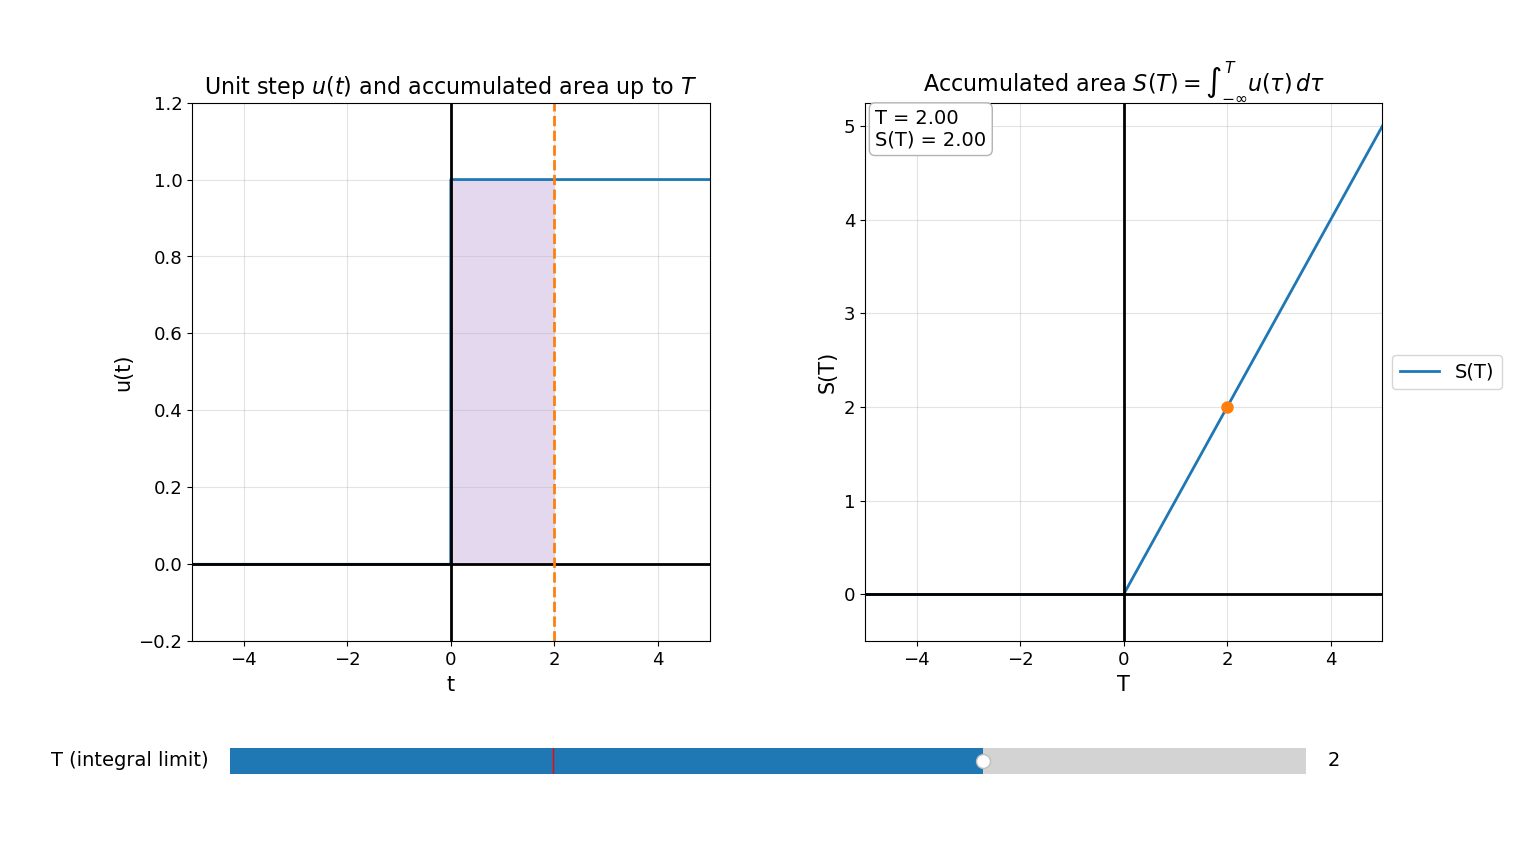
\includegraphics[width=\textwidth]{figs/unit_step_accumulator.png}
    \caption{The unit step function $u(t)$ (left) and its accumulated area, the ramp function $r(t)$ (right). The slider below sets the upper limit of integration $T$.}
    \label{fig:unit_accumulator}
\end{figure}
This ramp function increases linearly for $t \geq 0$ and is zero for $t < 0$. It effectively accumulates the area under the unit step function. See Figure~\ref{fig:unit_accumulator} for a sketch of the unit step function and its accumulated area (the ramp function) on the right side. A virtual manipulative is available for you to explore this concept interactively on the course Github page\footnote{Here is the \href{https://github.com/ee-ucmerced/ee102-signals-systems/tree/main/lecture\_notes/week2\_signal\_properties/VM\_unit\_step\_accumulator.py}{link} for virtual manipulative on Github for unit step as an accumulator}.
\section{The unit impulse function}
The unit impulse function is our second of the ``timeless trio'' of signals --- one of the three most important signals in signal processing. In other fields, such as physics, it is also known as the Dirac delta function. In discrete mathematics, it is known as the Kronecker delta function. So, the same mysterious function has many different names! The reason is clear --- it is a very useful mathematical object, while not even being a function in the traditional sense! We will define it formally later, but for now, let's understand it informally. You only need to remember two properties about the impulse function:
\begin{itemize}
    \item It is zero at all times except at $t = 0$, that is $\delta(t) = 0$ for all $t \neq 0$.
    \item It has an area of 1 under its curve, that is, $\int_{-\infty}^{\infty} \delta(t) dt = 1$.
\end{itemize}
How is that possible? If a signal is zero everywhere except at one point, then there must be something unique happening at that point. To build intuition for this function, consider the rectangular pulse we defined earlier, with a slight modification. Let's define a rectangular pulse of width $\epsilon$ and height $\frac{1}{\epsilon}$ around the origin:
\[
p_\epsilon(t) = \frac{1}{\epsilon} \left[u\left(t + \frac{\epsilon}{2}\right) - u\left(t - \frac{\epsilon}{2}\right)\right].
\]
A sketch of this pulse is shown in Figure~\ref{fig:impulse_approx}. 
\begin{figure}[h!]
  \centering
  % numeric epsilon used for drawing; labels will show symbols (±\epsilon/2, 1/\epsilon)
  \pgfmathsetmacro{\eps}{1.0}       % <-- choose the width \epsilon here
  \pgfmathsetmacro{\amp}{1/\eps}    % height = 1/\epsilon
  \begin{tikzpicture}
    \begin{axis}[
      axis lines=middle,
      axis line style={line width=1pt},
      xlabel={$t$},
      ylabel={$p_\epsilon(t)$},
      % x-ticks: show 0 normally, and symbolic ±\epsilon/2 as extra ticks
      xtick={0},
      extra x ticks={-0.5*\eps, 0.5*\eps},
      extra x tick labels={$-\frac{\epsilon}{2}$, $\frac{\epsilon}{2}$},
      % y-ticks: show 0 normally, and symbolic 1/\epsilon as extra tick
      ytick={0},
      extra y ticks={\amp},
      extra y tick labels={$\,\frac{1}{\epsilon}$},
      ymin={-0.15*\amp}, ymax={1.25*\amp},
      xmin={-2.2*\eps},  xmax={ 2.2*\eps},
      grid=both,
      width=10cm,
      height=6cm,
      samples=800,
    ]
      % rectangular pulse: height 1/eps on [-eps/2, eps/2), zero elsewhere
      \addplot[thick,blue,domain=-2.2*\eps:2.2*\eps]
        { (abs(x) <= 0.5*\eps) * \amp };

      % dashed guides at ±\epsilon/2
      \draw[dashed] (axis cs:-0.5*\eps,0) -- (axis cs:-0.5*\eps,\amp);
      \draw[dashed] (axis cs: 0.5*\eps,0) -- (axis cs: 0.5*\eps,\amp);
    \end{axis}
  \end{tikzpicture}
  \caption{Rectangular pulse $p_\epsilon(t)=\tfrac{1}{\epsilon}\!\left[u\!\left(t+\tfrac{\epsilon}{2}\right)-u\!\left(t-\tfrac{\epsilon}{2}\right)\right]$ of width $\epsilon$ centered at the origin.}
  \label{fig:impulse_approx}
\end{figure}

As you can see in the figure, the area of the rectangle is equal to 1 for all values of $\epsilon$. But this does not satisfy the two properties of the impulse function listed above as there are points $t \neq 0$ where the pulse is non-zero. So, we need to modify this pulse further. As we make $\epsilon$ smaller, visualize how the rectangle becomes taller and narrower, while still maintaining an area of 1. You can interactively explore this concept using the virtual manipulative available on the course Github page\footnote{Here is the \href{https://github.com/ee-ucmerced/ee102-signals-systems/tree/main/lecture\_notes/week2\_signal\_properties/VM\_delta\_via\_pulse.py}{link} for virtual manipulative on Github for impulse approximation using a pulse. Additionally, you can approximate an impulse using a Gaussian function, see \href{https://github.com/ee-ucmerced/ee102-signals-systems/tree/main/lecture\_notes/week2\_signal\_properties/VM\_delta\_via\_gaussian.py}{here}.}.

\subsection{Impulse as the limit of a rectangular pulse}
Formally, we can write the unit impulse function as the limit of the rectangular pulse as $\epsilon$ approaches zero:
\[
\delta(t) = \lim_{\epsilon \to 0} p_\epsilon(t) = \lim_{\epsilon \to 0} \frac{1}{\epsilon} \left[u\left(t + \frac{\epsilon}{2}\right) - u\left(t - \frac{\epsilon}{2}\right)\right].
\]
Despite the definition above, it is not possible to write a closed-form expression for the impulse function because it is not defined at $t = 0$ and is zero everywhere else. The only quantifiable property that we know so far is that the area under the curve of a delta function is equal to 1. To visually describe an impulse function, we draw an arrow pointing upwards at the point at which the impuse is located. That is, if we have $\delta(t)$, we draw an arrow at $t = 0$; if we have $\delta(t - t_0)$, we draw an arrow at $t = t_0$. The height of the arrow is not important, but we label it with a number to indicate the area under the impulse. For example, if we have $A \delta(t - t_0)$, we draw an arrow at $t = t_0$ and label it with $A$ to indicate that the area under the impulse is equal to $A$.

In practice, we can never generate a true impulse function, we can only get infinitesimally close to it as we keep making the width of the rectangular pulse infinitesimally close to zero and the height of the pulse close to infinity. Even though this may sound needlessly confusing, it provides us with a very powerful mathematical tool. One example is discussed next.
\subsection{Impulse as a time-sampler}
The impulse function can sample any test function at a specific point in time. Note that if we write $f(t)\delta(t)$, the product will be zero for all $t \neq 0$ because $\delta(t)$ is zero for all $t \neq 0$. The only point where the product is non-zero is at $t = 0$. So we can write $f(t)\delta(t) = f(0)\delta(t)$. This is also an impulse function located at $t = 0$ with an area of $f(0)$. Now if we integrate this product over all time, we get
\[\int_{-\infty}^{\infty} f(t) \delta(t) dt = f(0) \int_{-\infty}^{\infty} \delta(t) dt = f(0) \cdot 1 = f(0).\]
This property is known as the sifting property of the impulse function. By integrating any test function multiplied by an impulse function, we can extract the value of the test function at the location of the impulse $\rightarrow$ we have sampled that function! More generally, if we have an impulse located at $t = t_0$, we can write this impulse as $\delta(t - t_0)$. Then, by the same reasoning as above, we can show that\
\[
f(t_0) = \int_{-\infty}^{\infty} f(t) \delta(t - t_0) \, dt.
\]
To prove the above, write the integral as
\[
\int_{-\infty}^{\infty} f(t) \delta(t - t_0) \, dt = f(t_0) \int_{-\infty}^{\infty} \delta(t - t_0) \, dt = f(t_0) \cdot 1 = f(t_0).
\]
We obtained the latter equality by observing that $\delta(t - t_0)$ is zero at every point other than $t = t_0$. Since $f(t_0)$ is independent of $t$, we can take it outside the integral. The remaining integral is equal to 1 because the area under the impulse function is equal to 1. This property makes the impulse function a powerful tool in signal processing and system analysis.

In formal mathematical analysis, the above is not seen as a property but is instead used to \emph{define} the impulse function.
\begin{definition}
The unit impulse function $\delta(t)$ is defined as the function for which the area under curve of its product with any test function $f(t)$ that is continuous at $t = 0$, is equal to the value of the test function at the time instant at which the impulse is located ($t = 0$ for $\delta(t)$). That is,
\begin{equation}
\label{eq:impulse_def}
    \int_{-\infty}^{\infty} f(t) \delta(t) dt = f(0).
\end{equation}

\end{definition}
\subsection{Relationship between unit step and unit impulse}
If you look back at the unit step function, you will notice that it is discontinuous at $t = 0$. So, can we define the differentiation of unit step function with time, $du/dt$? Generally, the answer will be no since the derivative of a function is not defined at points where the function is discontinuous. Let's try an alternate approach. Consider the following integral:
\[
\int_{-\infty}^{\infty} f(t)\frac{du(t)}{dt}  dt.
\]
We can evaluate this integral using integration by parts to write
\begin{align*}
\int_{-\infty}^{\infty} f(t)\frac{du(t)}{dt}  dt &= f(t)u(t)\big|_{-\infty}^{\infty} - \int_{-\infty}^{\infty} u(t) \frac{df(t)}{dt} dt\\
&= f(\infty) - \int_{0}^{\infty} \frac{df(t)}{dt} dt\\
&= f(\infty) - [f(t)]_{0}^{\infty}\\
&= f(\infty) - f(\infty) + f(0).
\end{align*}
So, we derived that 
\begin{equation}
    \label{eq:du_dt}
    \int_{-\infty}^{\infty} f(t)\frac{du(t)}{dt}  dt = f(0),
\end{equation}
which is the same as the definition of the impulse function discussed earlier --- the area under the product of any test function and the impulse function is equal to the value of the test function at the location of the impulse. So, we can conclude by comparing equations~\eqref{eq:impulse_def} and~\eqref{eq:du_dt} that 
\[
\frac{du(t)}{dt} = \delta(t).
\]
Using a similar approach, you can also show that (HW \#2)
\[
u(t) = \int_{-\infty}^{t} \delta(\tau) d\tau.
\]
\section{Complex exponential signals}
\subsection*{Continuous time}
\[
x(t)=A\,e^{j(\omega_0 t+\phi)}=A\cos(\omega_0 t+\phi)+j\,A\sin(\omega_0 t+\phi).
\]
Real and imaginary parts are orthogonal sinusoids. Fundamental period $T_0=\frac{2\pi}{\omega_0}$.

\subsection*{Discrete time}
\[
x[n]=A\,e^{j(\Omega_0 n+\phi)}.
\]
This is periodic iff $\dfrac{\Omega_0}{2\pi}=\dfrac{M}{N}$ with integers $M,N$ coprime. Then the fundamental period is $N_0=N$. Otherwise, it is \emph{aperiodic} on $\mathbb{Z}$.

\subsection*{Geometric phasor}
The complex exponential traces a circle of radius $A$ in the complex plane at angular speed $\omega_0$ (continuous) or advances by a fixed angle $\Omega_0$ per sample (discrete). The real part is the projection on the horizontal axis and the imaginary part is the vertical projection.
% \section{The unit impulse function $\delta(t)$}
% See notes \url{https://ocw.mit.edu/courses/es-1803-differential-equations-spring-2024/mites_1803_s24_topic20.pdf}
\end{document}